\chapter{Results}
In the following, we present the results we obtained by answering the Key Analytical Questions defined in Chapter \ref{ch:2} using the data warehouse designed and implemented in the previous chapters. For that, we executed the queries defined for each question against the data warehouse and visualized the results using appropriate charts.

\paragraph{How does user engagement evolve over multiple subscription tiers over time?}
For our first question, we wanted to know how the user engagement evolves over multiple subscription tiers. But it is also helpful to see how engagement evolves over time in general, so we can spot trends and seasonality. Therefore, we created a query that aggregates the number of active users per month and subscription tier. Furthermore, we also wanted to see how many active users are in each tier in total over the time span, so we can see, which tier has the most engagement. Finally, we wanted to know what the total engagement was over the total time span to see how many users were active in total. To extract those information, we used the query described in Listing \ref{lst:kaq1}.
\begin{lstlisting}[language=SQL,caption={Query for answering: How does user engagement evolve over time across subsciption tiers?},label={lst:kaq1},captionpos=b]
SELECT t.year, t.month, u.subscription_tier,
  SUM(f.active_user_flag) AS dau,
FROM fact_product_usage_engagement f
JOIN dim_time t ON t.time_key = f.time_key
JOIN dim_user u ON u.user_key = f.user_key
GROUP BY GROUPING SETS (
  (t.year, t.month, u.subscription_tier),
  (t.year, t.month),
  (u.subscription_tier),
  ()
)
ORDER BY t.year NULLS LAST, t.month NULLS LAST,
                u.subscription_tier NULLS LAST;
\end{lstlisting}

To retrieve the data we wanted to know, it was benefitial to use the \texttt{GROUPING SETS} feature of SQL, which allows us to group by multiple dimensions in a single query. This way, we could get the monthly active users per subscription tier, the total active users per subscription tier, and the total active users overall in a single query. After executing the query against our data warehouse, we visualized the results of the evolution of user engagement over time in Figure \ref{fig:kaq1}.
\begin{figure}[H]
    \centering
    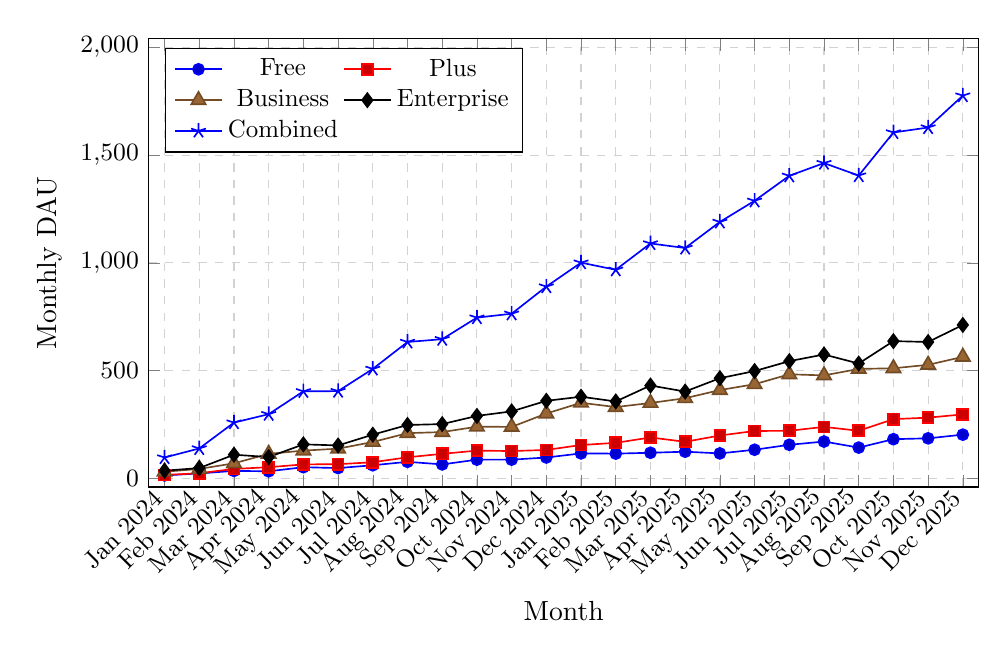
\begin{tikzpicture}
        \begin{axis}[
            width=\textwidth,
            height=0.6\textwidth,
            xlabel={Month},
            ylabel={Monthly DAU},
            xmin=1,
            xmax=24,
            ymin=0,
            ymax=2000,
            xtick={1,...,24},
            xticklabels={
                Jan 2024,Feb 2024,Mar 2024,Apr 2024,May 2024,Jun 2024,
                Jul 2024,Aug 2024,Sep 2024,Oct 2024,Nov 2024,Dec 2024,
                Jan 2025,Feb 2025,Mar 2025,Apr 2025,May 2025,Jun 2025,
                Jul 2025,Aug 2025,Sep 2025,Oct 2025,Nov 2025,Dec 2025
            },
            xticklabel style={rotate=45, anchor=east},
            tick label style={font=\small},
            legend style={at={(0.02,0.98)}, anchor=north west, nodes={scale=0.9, transform shape}},
            legend columns=2,
            grid=both,
            major grid style={dashed, gray!35},
            minor grid style={dotted, gray!20},
            enlargelimits=0.02,
            unbounded coords=discard
        ]
            \addplot+[semithick, mark=*, mark size=2pt] coordinates {
                (1, 14) (2, 23) (3, 35) (4, 33) (5, 52) (6, 48)
                (7, 61) (8, 77) (9, 65) (10, 87) (11, 87) (12, 97)
                (13, 116) (14, 115) (15, 119) (16, 124) (17, 116) (18, 133)
                (19, 156) (20, 171) (21, 143) (22, 182) (23, 186) (24, 203)
            };
            \addplot+[semithick, mark=square*, mark size=2pt] coordinates {
                (1, 16) (2, 24) (3, 44) (4, 52) (5, 65) (6, 66)
                (7, 75) (8, 98) (9, 114) (10, 129) (11, 127) (12, 132)
                (13, 155) (14, 165) (15, 190) (16, 170) (17, 199) (18, 220)
                (19, 221) (20, 239) (21, 221) (22, 275) (23, 282) (24, 297)
            };
            \addplot+[semithick, mark=triangle*, mark size=3pt] coordinates {
                (1, 31) (2, 44) (3, 70) (4, 114) (5, 129) (6, 138)
                (7, 169) (8, 210) (9, 215) (10, 240) (11, 239) (12, 301)
                (13, 351) (14, 331) (15, 350) (16, 372) (17, 410) (18, 437)
                (19, 483) (20, 478) (21, 508) (22, 511) (23, 527) (24, 564)
            };
            \addplot+[semithick, mark=diamond*, mark size=2.5pt] coordinates {
                (1, 36) (2, 48) (3, 110) (4, 99) (5, 158) (6, 153)
                (7, 203) (8, 248) (9, 252) (10, 290) (11, 311) (12, 360)
                (13, 379) (14, 357) (15, 431) (16, 403) (17, 465) (18, 498)
                (19, 544) (20, 575) (21, 533) (22, 637) (23, 633) (24, 712)
            };
            \addplot+[semithick, mark=star, mark size=2.8pt] coordinates {
                (1, 97) (2, 139) (3, 259) (4, 298) (5, 404) (6, 405)
                (7, 508) (8, 633) (9, 646) (10, 746) (11, 764) (12, 890)
                (13, 1001) (14, 968) (15, 1090) (16, 1069) (17, 1190) (18, 1288)
                (19, 1404) (20, 1463) (21, 1405) (22, 1605) (23, 1628) (24, 1776)
            };
            \legend{Free, Plus, Business, Enterprise, Combined}
        \end{axis}
    \end{tikzpicture}
    \caption{Monthly DAU by subscription tier for Jan 2024--Dec 2025.}
    \label{fig:kaq1-dau}
\end{figure}

To compare the total engagement per subscription tier, we created a bar chart as shown in Figure \ref{fig:kaq1-total}.
\begin{figure}[H]
    \centering
    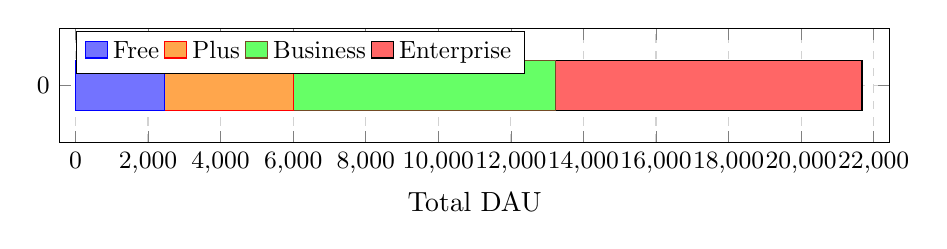
\begin{tikzpicture}
        \begin{axis}[
            xbar stacked,
            width=\textwidth,
            height=0.25\textwidth,
            xlabel={Total DAU},
            ytick={0},
            xmin=0,
            xmax=22000,
            scaled ticks=false,
            bar width=18pt,
            tick label style={font=\small},
            legend style={at={(0.02,0.98)}, anchor=north west, nodes={scale=0.9, transform shape}},
            legend columns=4,
            grid=both,
            major grid style={dashed, gray!35},
            minor grid style={dotted, gray!20},
            enlargelimits=0.02
        ]
            \addplot+[fill=blue!55] coordinates {(2443, 0)};
            \addplot+[fill=orange!70] coordinates {(3576, 0)};
            \addplot+[fill=green!60] coordinates {(7222, 0)};
            \addplot+[fill=red!60] coordinates {(8435, 0)};
            \legend{Free, Plus, Business, Enterprise}
        \end{axis}
    \end{tikzpicture}
    \caption{Total DAU by subscription tier for Jan 2024 - Dec 2025.}
    \label{fig:kaq1-total}
\end{figure}

Here we can see that the \textit{Enterprise} tier has the highest total daily active users (DAU) with 8,435 users, followed by the \textit{Business} tier with 7,222 users. The \textit{Plus} and \textit{Free} tiers have significantly lower total DAU, with 3,576 and 2,443 users respectively. This indicates that higher subscription tiers tend to have more engaged users, which could be due to the higher involvement they have do to higher billing plans. To get a better understanding of the user engagement we take a look at the second question.

\paragraph{Which content types generate the highest sustained interaction rates?}
To answer our second question, we wanted to know which content types generate the highest sustained interaction rates. Therefore, we created a query that aggregates the number of interactions per content type and month. This way, we can see which content types are interacted with the most over time. To extract those information, we used the query described in Listing \ref{lst:kaq2}.
\begin{lstlisting}[language=SQL,caption={Query for answering: How does user engagement evolve over time across subsciption tiers?},label={lst:kaq2},captionpos=b]
SELECT t.year, t.month, c.content_type,
        SUM(f.active_user_flag) AS dau
FROM fact_product_usage_engagement f
JOIN dim_time t    ON t.time_key = f.time_key
JOIN dim_content c ON c.content_key = f.content_key
GROUP BY CUBE (t.year, t.month, c.content_type)
ORDER BY t.year NULLS LAST, t.month NULLS LAST,
                    c.content_type NULLS LAST;
\end{lstlisting}

This time, we used \texttt{CUBE} to retrieve all combinations of content types, months and years. This way, we could get all levels of granularity in a single query. Therefore, we can get a little bit more insights into the data which is especially benefitial when investigating content types. First, we take a look at the usage of the diffrent content types over time as shown in Figure \ref{fig:kaq2}.
\begin{figure}[H]
    \centering
    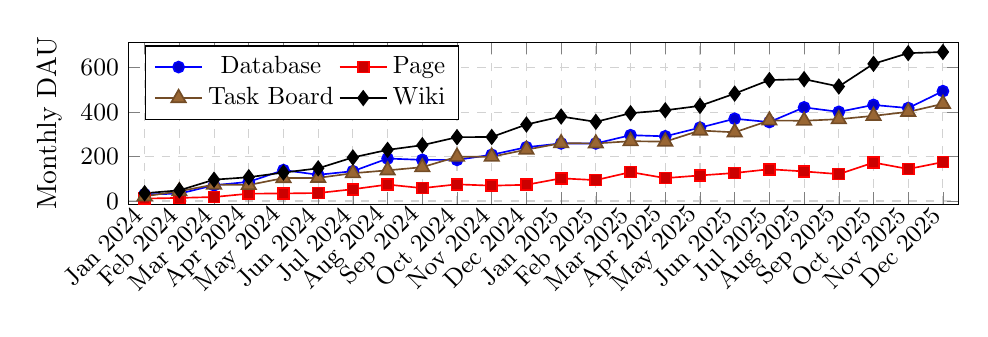
\begin{tikzpicture}
        \begin{axis}[
            width=\textwidth,
            height=0.3\textwidth,
            ylabel={Monthly DAU},
            xmin=1,
            xmax=24,
            ymin=0,
            ymax=700,
            xtick={1,...,24},
            xticklabels={
                Jan 2024,Feb 2024,Mar 2024,Apr 2024,May 2024,Jun 2024,
                Jul 2024,Aug 2024,Sep 2024,Oct 2024,Nov 2024,Dec 2024,
                Jan 2025,Feb 2025,Mar 2025,Apr 2025,May 2025,Jun 2025,
                Jul 2025,Aug 2025,Sep 2025,Oct 2025,Nov 2025,Dec 2025
            },
            xticklabel style={rotate=45, anchor=east},
            tick label style={font=\small},
            legend style={at={(0.02,0.98)}, anchor=north west, nodes={scale=0.9, transform shape}},
            legend columns=2,
            grid=both,
            major grid style={dashed, gray!35},
            minor grid style={dotted, gray!20},
            enlargelimits=0.02,
            unbounded coords=discard
        ]
            \addplot+[semithick, mark=*, mark size=2pt] coordinates {
                (1, 30) (2, 33) (3, 71) (4, 86) (5, 139) (6, 118)
                (7, 134) (8, 191) (9, 185) (10, 185) (11, 208) (12, 242)
                (13, 259) (14, 259) (15, 296) (16, 291) (17, 330) (18, 370)
                (19, 355) (20, 421) (21, 401) (22, 432) (23, 418) (24, 494)
            };
            \addplot+[semithick, mark=square*, mark size=2pt] coordinates {
                (1, 11) (2, 14) (3, 18) (4, 33) (5, 34) (6, 36)
                (7, 53) (8, 74) (9, 58) (10, 75) (11, 69) (12, 73)
                (13, 102) (14, 94) (15, 130) (16, 103) (17, 115) (18, 126)
                (19, 143) (20, 133) (21, 121) (22, 173) (23, 144) (24, 175)
            };
            \addplot+[semithick, mark=triangle*, mark size=3pt] coordinates {
                (1, 21) (2, 44) (3, 74) (4, 72) (5, 103) (6, 104)
                (7, 125) (8, 138) (9, 152) (10, 199) (11, 199) (12, 231)
                (13, 260) (14, 259) (15, 269) (16, 267) (17, 317) (18, 309)
                (19, 362) (20, 361) (21, 368) (22, 383) (23, 401) (24, 437)
            };
            \addplot+[semithick, mark=diamond*, mark size=2.5pt] coordinates {
                (1, 35) (2, 48) (3, 96) (4, 107) (5, 128) (6, 147)
                (7, 196) (8, 230) (9, 251) (10, 287) (11, 288) (12, 344)
                (13, 380) (14, 356) (15, 395) (16, 408) (17, 428) (18, 483)
                (19, 544) (20, 548) (21, 515) (22, 617) (23, 665) (24, 670)
            };
            \legend{Database, Page, Task Board, Wiki}
        \end{axis}
    \end{tikzpicture}
    \caption{Monthly DAU by content type for Jan 2024 - Dec 2025.}
    \label{fig:kaq2}
\end{figure}

Here we can see that the \textit{Wiki} content type has the highest monthly DAU, followed by \textit{Task Board}, \textit{Database}, and \textit{Page}. This indicates that users tend to interact more with \textit{Wiki} content, which could be due to its collaborative nature and the fact that it is often used for documentation and knowledge sharing. To highlight seasonal patterns independent of year-to-year growth, we aggregated monthly DAU across years for each content type. In Figure \ref{fig:kaq2-seasonality}, we can see the seasonality of each content type.
\begin{figure}[H]
    \centering
    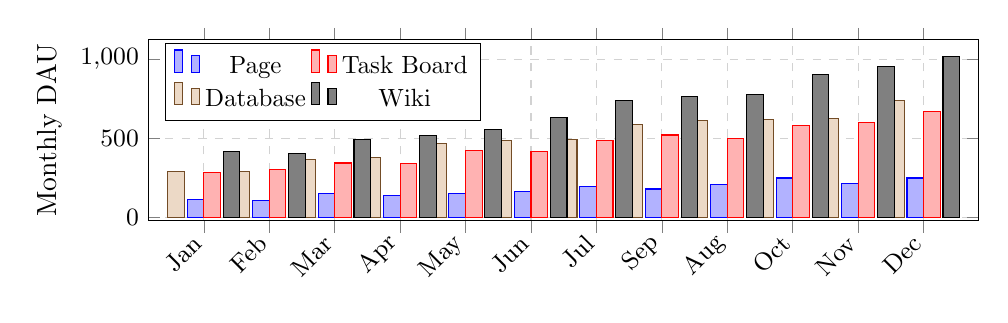
\begin{tikzpicture}
        \begin{axis}[
            width=\textwidth,
            height=0.32\textwidth,
            ybar,
            bar width=6pt,
            ylabel={Monthly DAU},
            ymin=0,
            ymax=1100,
            xmin=0.4,
            xmax=12.6,
            xtick={1,...,12},
            xticklabels={Jan,Feb,Mar,Apr,May,Jun,Jul,Sep,Aug,Oct,Nov,Dec},
            xticklabel style={rotate=45, anchor=east},
            tick label style={font=\small},
            legend style={at={(0.02,0.98)}, anchor=north west, nodes={scale=0.9, transform shape}},
            legend columns=2,
            grid=both,
            major grid style={dashed, gray!35},
            minor grid style={dotted, gray!20},
            enlargelimits=0.02,
            unbounded coords=discard
        ]
            \addplot+[bar shift=-3pt] coordinates {
                (1, 113) (2, 108) (3, 148) (4, 136) (5, 149) (6, 162)
                (7, 196) (8, 179) (9, 207) (10, 248) (11, 213) (12, 248)
            };
            \addplot+[bar shift=3pt] coordinates {
                (1, 281) (2, 303) (3, 343) (4, 339) (5, 420) (6, 413)
                (7, 487) (8, 520) (9, 499) (10, 582) (11, 600) (12, 668)
            };
            \addplot+[bar shift=-10pt] coordinates {
                (1, 289) (2, 292) (3, 367) (4, 377) (5, 469) (6, 488)
                (7, 489) (8, 586) (9, 612) (10, 617) (11, 626) (12, 736)
            };
            \addplot+[bar shift=10pt] coordinates {
                (1, 415) (2, 404) (3, 491) (4, 515) (5, 556) (6, 630)
                (7, 740) (8, 766) (9, 778) (10, 904) (11, 953) (12, 1014)
            };
            \legend{Page, Task Board, Database, Wiki}
        \end{axis}
    \end{tikzpicture}
    \caption{Seasonality by month across years (aggregated over 2024 - 2025).}
    \label{fig:kaq2-seasonality}
\end{figure}

As we can see, no content type shows a significant seasonal pattern. Since we aggregated the data across years, the dip we saw earlier in September is not visible anymore. Overall, we can conclude that \textit{Wiki} and \textit{Task Board} content types generate the highest sustained interaction rates, while \textit{Page} content has the lowest engagement. To see if the content types with the highest daily active users also have the highest event count we run the query shown in Listing \ref{lst:kaq2-events}.
\begin{lstlisting}[language=SQL,caption={Query for answering: How does user engagement evolve over time across different content types?},label={lst:kaq2-events},captionpos=b]
SELECT
  c.content_type,
  SUM(f.event_count) AS events,
  DENSE_RANK() OVER (ORDER BY SUM(f.event_count) DESC)
                                AS content_type_rank
FROM fact_product_usage_engagement f
JOIN dim_content c ON c.content_key = f.content_key
GROUP BY c.content_type
ORDER BY content_type_rank, c.content_type;
\end{lstlisting}

After executing the query against our data warehouse, we visualized the results in Table \ref{tab:kaq2-events}.
\begin{table}[H]
\centering
\begin{tabular}{lcc}
\hline
\textbf{Content Type} & \textbf{Events} & \textbf{Rank} \\
\hline
wiki & $40719$ & $1$ \\
database & $30393$ & $2$ \\
task\_board & $26982$ & $3$ \\
page & $10544$ & $4$ \\
\hline
\end{tabular}
\caption{Resulting table after running the query in Listing \ref{lst:kaq2-events}.}\label{tbl:kaq2-events}
\end{table}

Here we can see that the \textit{Wiki} content type has the highest event count with 40,719 events, followed by \textit{Database} with 30,393 events, \textit{Task Board} with 26,982 events, and \textit{Page} with 10,544 events. This indicates that the content types with the highest daily active users also tend to have the highest event counts, suggesting a strong correlation between user engagement and interaction frequency. Overall, we can conclude that \textit{Wiki} and \textit{Database} content types not only generate the highest sustained interaction rates but also have the highest event counts. This information can be used to inform product development and marketing strategies, as well as to identify areas for improvement in user engagement. Now we take a look at the activation rates of new users.

\paragraph{What are the activation rates of new users within their first seven days?}
To answer our third question, we wanted to know what the activation rates of new users are within their first seven days. Therefore, we created a query that calculates the percentage of new users who become active within their first seven days after sign-up. To extract those information, we used the query described in Listing \ref{lst:kaq3}.
\begin{lstlisting}[language=SQL,caption={Query for answering: How does user engagement evolve over time across subsciption tiers?},label={lst:kaq3},captionpos=b]
WITH user_events AS (
  SELECT
    u.user_key,
    u.signup_date,
    t.calendar_date,
    f.activation_event_flag,
    ROW_NUMBER() OVER w AS rn_after_signup
  FROM fact_product_usage_engagement f
  JOIN dim_user u ON u.user_key = f.user_key
  JOIN dim_time t ON t.time_key = f.time_key
  WHERE t.calendar_date >= u.signup_date
    AND t.calendar_date <  u.signup_date + INTERVAL '7 days'
  WINDOW w AS 
    (PARTITION BY u.user_key ORDER BY t.calendar_date)
),
activation_by_user AS (
  SELECT
    user_key,
    MIN(signup_date) AS signup_date,
    MAX(activation_event_flag) AS activated_within_7d
  FROM user_events
  GROUP BY user_key
)
SELECT
  DATE_TRUNC('month', signup_date)::date AS signup_month,
  COUNT(*)                               AS new_users,
  SUM(activated_within_7d)               AS activated_users,
  ROUND(
    SUM(activated_within_7d)::numeric / NULLIF(COUNT(*), 0),
    4
  )                                      AS activation_rate
FROM activation_by_user
GROUP BY DATE_TRUNC('month', signup_date)
ORDER BY signup_month;
\end{lstlisting}

In this query, we first created a Common Table Expression (CTE) called \texttt{user\_events} that retrieves all user events within the first seven days after sign-up. We then created another CTE called \texttt{activation\_by\_user} that aggregates the data by user and determines whether each user activated within the seven-day window. Finally, we calculated the activation rate by dividing the number of activated users by the total number of new users for each month. After executing the query against our data warehouse, we visualized the results in Figure \ref{fig:kaq3}.
\def\MonthTickLabels{2024-01,2024-02,2024-03,2024-04,2024-05,2024-06,2024-07,2024-08,2024-09,2024-10,2024-11,2024-12,2025-01,2025-02,2025-03,2025-04,2025-05,2025-06,2025-07,2025-08,2025-09,2025-10,2025-11,2025-12}

\pgfplotstableread[col sep=comma]{../../results/kaq3.csv}\kaqthreedata

\begin{figure}[H]
\centering
\begin{tikzpicture}
\begin{axis}[
    name=kaqthree,
    width=\textwidth,
    height=8cm,
    ybar,
    bar width=10pt,
    ymin=0,
    xtick={0,...,23},
    xticklabels={\MonthTickLabels},
    xticklabel style={rotate=45, anchor=east},
    ylabel={Users},
    legend style={at={(0.02,0.98)}, anchor=north west, cells={anchor=west}},
    grid=both,
    major grid style={gray!30},
    minor grid style={gray!15},
]
    \addplot+[fill=blue!50]
        table[
            x expr=\coordindex,
            y=new_users
        ] {\kaqthreedata};
    \addlegendentry{New users}

    \addplot+[fill=green!60!black]
        table[
            x expr=\coordindex,
            y=activated_users
        ] {\kaqthreedata};
    \addlegendentry{Activated users}
\end{axis}

\begin{axis}[
    at={(kaqthree.south west)},
    anchor=south west,
    width=\textwidth,
    height=8cm,
    axis x line=none,
    axis y line*=right,
    ymin=0,
    ymax=1,
    yticklabel style={color=orange!80!black},
    ylabel={Activation rate},
    y label style={color=orange!80!black},
    xtick={0,...,23},
    xticklabels=\empty,
    legend style={at={(0.98,0.98)}, anchor=north east},
]
    \addplot+[thick, color=orange!80!black, mark=*]
        table[
            x expr=\coordindex,
            y=activation_rate
        ] {\kaqthreedata};
    \addlegendentry{Activation rate}
\end{axis}
\end{tikzpicture}
\caption{New users, activations, and activation rate by signup month (kaq3).}
\label{fig:kaq3}
\end{figure}

Here we can see that the activation rate of new users within their first seven days fluctuates between approximately 0.6 and 0.9 over the observed period. There is a noticable dip in mid 2024 with the exception of September 2024, where the activation rate drops to around 0.6. After that, the activation rate gradually increases again, reaching a peak of around 0.9 in May 2025 and after that it stabelizes between 0.7 and 0.85. Overall, we can conclude that the activation rates of new users within their first seven days show some fluctuations over time, but generally tend to be relatively high. This information can be used to inform user onboarding strategies and identify areas for improvement in the activation process. Next, we take a look on how devices influences the user activity and session duration.
\paragraph{How does device usage affect user activity and session duration?}
Now, to answer our fourth question, we wanted to know how device usage affects user activity and session duration. Therefore, we created a query that aggregates the number of active users and average session duration per device type and month. This way, we can see how different devices impact user engagement over time. To extract those information, we used the query described in Listing \ref{lst:kaq4}.
\input{../listings/kaq4-query}
In this query, we joined the fact table with the time and device dimension tables to retrieve the necessary information. We then grouped the data by year, month, and device platform using the \texttt{ROLLUP} feature to get all levels of granularity in a single query. After executing the query against our data warehouse, we visualized the results of user activity over time by device type in Figure \ref{fig:kaq4-activity}.
\begin{figure}[H]
    \centering
    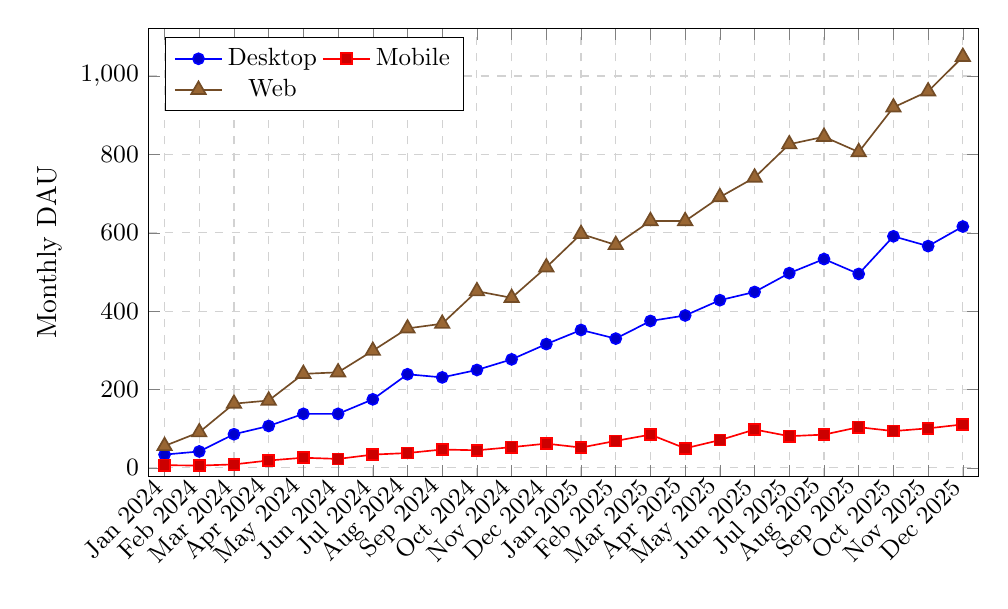
\begin{tikzpicture}
        \begin{axis}[
            width=\textwidth,
            height=0.6\textwidth,
            ylabel={Monthly DAU},
            xmin=1,
            xmax=24,
            ymin=0,
            ymax=1100,
            xtick={1,...,24},
            xticklabels={
                Jan 2024,Feb 2024,Mar 2024,Apr 2024,May 2024,Jun 2024,
                Jul 2024,Aug 2024,Sep 2024,Oct 2024,Nov 2024,Dec 2024,
                Jan 2025,Feb 2025,Mar 2025,Apr 2025,May 2025,Jun 2025,
                Jul 2025,Aug 2025,Sep 2025,Oct 2025,Nov 2025,Dec 2025
            },
            xticklabel style={rotate=45, anchor=east},
            tick label style={font=\small},
            legend style={at={(0.02,0.98)}, anchor=north west, nodes={scale=0.9, transform shape}},
            legend columns=2,
            grid=both,
            major grid style={dashed, gray!35},
            minor grid style={dotted, gray!20},
            enlargelimits=0.02,
            unbounded coords=discard
        ]
            \addplot+[semithick, mark=*, mark size=2pt] coordinates {
                (1, 34) (2, 42) (3, 86) (4, 107) (5, 138) (6, 138)
                (7, 175) (8, 239) (9, 231) (10, 250) (11, 277) (12, 316)
                (13, 352) (14, 330) (15, 375) (16, 389) (17, 428) (18, 449)
                (19, 497) (20, 533) (21, 495) (22, 591) (23, 566) (24, 616)
            };
            \addplot+[semithick, mark=square*, mark size=2pt] coordinates {
                (1, 7) (2, 6) (3, 9) (4, 19) (5, 26) (6, 23)
                (7, 34) (8, 38) (9, 47) (10, 45) (11, 53) (12, 62)
                (13, 52) (14, 69) (15, 85) (16, 50) (17, 71) (18, 98)
                (19, 81) (20, 85) (21, 104) (22, 94) (23, 101) (24, 111)
            };
            \addplot+[semithick, mark=triangle*, mark size=3pt] coordinates {
                (1, 56) (2, 91) (3, 164) (4, 172) (5, 240) (6, 244)
                (7, 299) (8, 356) (9, 368) (10, 451) (11, 434) (12, 512)
                (13, 597) (14, 569) (15, 630) (16, 630) (17, 691) (18, 741)
                (19, 826) (20, 845) (21, 806) (22, 920) (23, 961) (24, 1049)
            };
            \legend{Desktop, Mobile, Web}
        \end{axis}
    \end{tikzpicture}
    \caption{Monthly DAU by device type for Jan 2024 - Dec 2025.}
    \label{fig:kaq4-activity}
\end{figure}

Here we can see that web users have the highest monthly DAU, followed by desktop and mobile users. This indicates that users tend to be more active on web platforms, which could be due to the convenience and accessibility of web applications. Desktop users also show a significant level of activity, while mobile users have the lowest monthly DAU. This could be due to the limitations of mobile devices, such as smaller screens and reduced functionality compared to desktop and web platforms. To get a better understanding of how device usage affects session duration, we visualized the average session duration per device type in Figure \ref{fig:kaq4-session-duration}.
\begin{figure}[H]
    \centering
    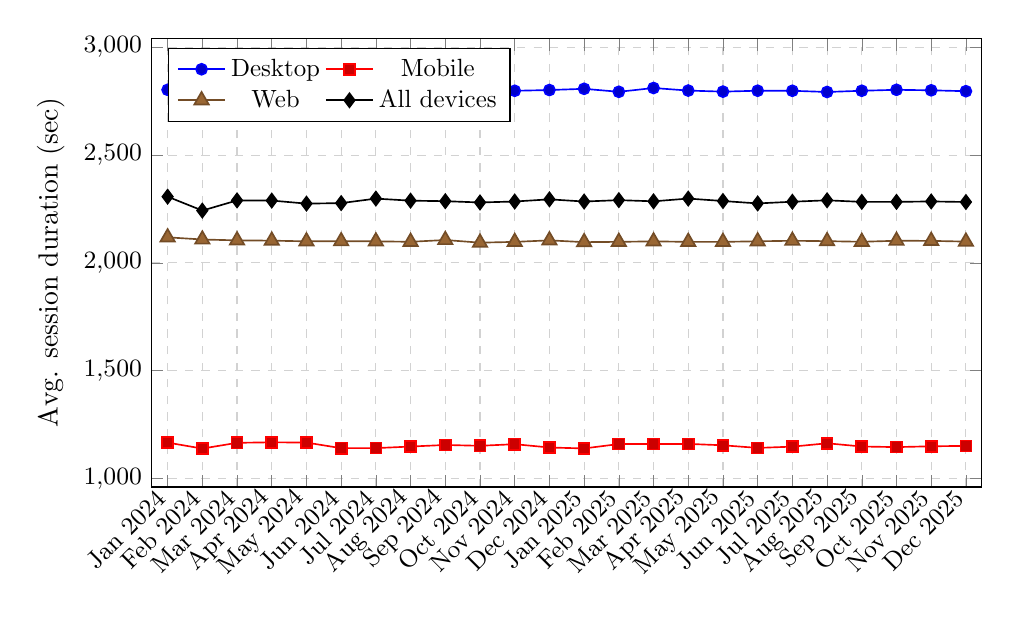
\begin{tikzpicture}
        \begin{axis}[
            width=\textwidth,
            height=0.6\textwidth,
            ylabel={Avg. session duration (sec)},
            xmin=1,
            xmax=24,
            ymin=1000,
            ymax=3000,
            xtick={1,...,24},
            xticklabels={
                Jan 2024,Feb 2024,Mar 2024,Apr 2024,May 2024,Jun 2024,
                Jul 2024,Aug 2024,Sep 2024,Oct 2024,Nov 2024,Dec 2024,
                Jan 2025,Feb 2025,Mar 2025,Apr 2025,May 2025,Jun 2025,
                Jul 2025,Aug 2025,Sep 2025,Oct 2025,Nov 2025,Dec 2025
            },
            xticklabel style={rotate=45, anchor=east},
            tick label style={font=\small},
            legend style={at={(0.02,0.98)}, anchor=north west, nodes={scale=0.9, transform shape}},
            legend columns=2,
            grid=both,
            major grid style={dashed, gray!35},
            minor grid style={dotted, gray!20},
            enlargelimits=0.02,
            unbounded coords=discard
        ]
            \addplot+[semithick, mark=*, mark size=2pt] coordinates {
                (1, 2802.9) (2, 2777.5) (3, 2781.7) (4, 2780.1) (5, 2794.6) (6, 2795.0)
                (7, 2817.7) (8, 2809.0) (9, 2807.7) (10, 2800.5) (11, 2798.4) (12, 2801.9)
                (13, 2807.6) (14, 2793.7) (15, 2811.3) (16, 2799.4) (17, 2794.5) (18, 2798.7)
                (19, 2798.4) (20, 2792.9) (21, 2798.5) (22, 2803.0) (23, 2800.6) (24, 2796.5)
            };
            \addplot+[semithick, mark=square*, mark size=2pt] coordinates {
                (1, 1166.1) (2, 1138.5) (3, 1165.2) (4, 1167.5) (5, 1166.3) (6, 1140.3)
                (7, 1140.6) (8, 1147.8) (9, 1155.2) (10, 1151.3) (11, 1158.8) (12, 1143.4)
                (13, 1139.1) (14, 1159.5) (15, 1159.3) (16, 1160.2) (17, 1153.7) (18, 1141.5)
                (19, 1147.4) (20, 1163.0) (21, 1148.0) (22, 1145.3) (23, 1149.0) (24, 1151.0)
            };
            \addplot+[semithick, mark=triangle*, mark size=3pt] coordinates {
                (1, 2118.5) (2, 2108.5) (3, 2104.4) (4, 2103.1) (5, 2099.9) (6, 2100.5)
                (7, 2099.9) (8, 2097.8) (9, 2106.1) (10, 2093.8) (11, 2097.4) (12, 2104.5)
                (13, 2096.2) (14, 2097.6) (15, 2099.8) (16, 2097.5) (17, 2097.5) (18, 2100.1)
                (19, 2102.6) (20, 2100.7) (21, 2097.9) (22, 2102.6) (23, 2102.1) (24, 2098.7)
            };
            \addplot+[semithick, mark=diamond*, mark size=2.5pt] coordinates {
                (1, 2307.3) (2, 2242.6) (3, 2289.8) (4, 2289.1) (5, 2274.9) (6, 2277.3)
                (7, 2298.2) (8, 2288.6) (9, 2286.2) (10, 2280.3) (11, 2284.7) (12, 2294.8)
                (13, 2284.6) (14, 2291.1) (15, 2285.6) (16, 2298.4) (17, 2287.0) (18, 2275.8)
                (19, 2283.7) (20, 2290.3) (21, 2283.0) (22, 2283.0) (23, 2285.0) (24, 2282.4)
            };
            \legend{Desktop, Mobile, Web, All devices}
        \end{axis}
    \end{tikzpicture}
    \caption{Average session duration by device type for Jan 2024 - Dec 2025.}
    \label{fig:kaq4-session-duration}
\end{figure}

This plots also shows that web users have the longest average session duration, followed by desktop and mobile users. This further supports the idea that web platforms provide a more engaging user experience, leading to longer sessions. Desktop users also have a relatively high average session duration, while mobile users have the shortest sessions. This could be due to the fact that mobile users often use apps for quick tasks and may not spend as much time on them compared to desktop and web platforms. But also that the desktop and web version is more handy. Overall, we can conclude that device usage has a significant impact on user activity and session duration, with web platforms showing the highest engagement levels. This information can be used to inform product development and marketing strategies, as well as to identify areas for improvement in user engagement across different devices. We now proceed to our last key analytical question.
\paragraph{What proportion of total activity originates from collaborative versus individual work?}
To answer our fifth and final question, we wanted to know what proportion of total activity originates from collaborative versus individual work. Therefore, we created a query that aggregates the number of active users and events based on whether the activity was collaborative or individual. To extract those information, we used the query described in Listing \ref{lst:kaq5}.
\input{../listings/kaq5-query}
In this query, we first created a Common Table Expression (CTE) called \texttt{base} that retrieves the number of events per month and work mode (collaborative or individual). We then created another CTE called \texttt{totals} that calculates the total number of events per month. Finally, we joined the two CTEs to calculate the proportion of events for each work mode by dividing the number of events by the total number of events for each month. After executing the query against our data warehouse, we visualized the results in Figure \ref{fig:kaq5}.
\def\MonthTickLabels{2024-01,2024-02,2024-03,2024-04,2024-05,2024-06,2024-07,2024-08,2024-09,2024-10,2024-11,2024-12,2025-01,2025-02,2025-03,2025-04,2025-05,2025-06,2025-07,2025-08,2025-09,2025-10,2025-11,2025-12}

\pgfplotstableread[col sep=comma]{../../results/kaq5.csv}\kaqfivedata

\begin{figure}[H]
\centering
\begin{tikzpicture}
\begin{axis}[
    width=\textwidth,
    height=8cm,
    ybar stacked,
    bar width=12pt,
    ymin=0,
    ymax=1,
    ylabel={Proportion of events},
    xtick={0,...,23},
    xticklabels={\MonthTickLabels},
    xticklabel style={rotate=45, anchor=east},
    legend style={at={(0.02,0.98)}, anchor=north west, cells={anchor=west}},
    grid=both,
    major grid style={gray!30},
    minor grid style={gray!15},
]
    \addplot+[fill=blue!55]
        table[
            x expr=\coordindex,
            y=proportion,
            row predicate/.code={
                \pgfplotstablegetelem{\pgfplotstablerow}{work_mode}\of{\kaqfivedata}
                \edef\mode{\pgfplotsretval}
                \ifnum\pdfstrcmp{\mode}{collaborative}=0
                \else
                    \pgfplotstableuserowfalse
                \fi
            }
        ] {\kaqfivedata};
    \addlegendentry{Collaborative}

    \addplot+[fill=orange!70]
        table[
            x expr=\coordindex,
            y=proportion,
            row predicate/.code={
                \pgfplotstablegetelem{\pgfplotstablerow}{work_mode}\of{\kaqfivedata}
                \edef\mode{\pgfplotsretval}
                \ifnum\pdfstrcmp{\mode}{individual}=0
                \else
                    \pgfplotstableuserowfalse
                \fi
            }
        ] {\kaqfivedata};
    \addlegendentry{Individual}
\end{axis}
\end{tikzpicture}
\caption{Collaboration vs individual work share over time (kaq5).}
\label{fig:kaq5}
\end{figure}

Here we can see that collaborative work consistently accounts for a higher proportion of total activity compared to individual work. The proportion of collaborative work ranges from approximately 70\% to 80\%, while individual work ranges from approximately 20\% to 30\%. There are almost none fluctuations over time and the overall trend indicates that collaborative work is the dominant mode of activity. This suggests that users tend to engage more in collaborative tasks, which could be due to the nature of the platform and its focus on teamwork and collaboration. Overall, we can conclude that a significant proportion of total activity originates from collaborative work, highlighting the importance of collaboration in driving user engagement on the platform. This information can be used to inform product development and marketing strategies, as well as to identify areas for improvement in fostering collaboration among users.
